\section{Simulation}
\rhead{Simulation}

Der erste Schritt ist ein Modell zu erstellen.
Dazu wird der Golfstrom in drei Zonen aufgeteilt. Die jeweiligen Polarregionen und der Äquator. Diese Zonen erhalten je eine Box.
Im laufe des Seminars wurden zwei Modelle erstellt. Der erste Ansatz war sehr lehrreich hatte aber  schlussendlich nichts mit dem realen Golfstrom gemeinsam. Der zweite Ansatz war erfolgreicher und der Golfstrom kann mit diesem Modell qualitativ simuliert werden.
In den folgenden zwei Kapiteln werden diese Zwei Modelle vorgestellt und die jeweiligen Resultate diskutiert.

\subsection{Zwei-Fluss Modell(1.Ansatz)}

In diesem Modell werden die Boxen jeweils durch Rohre verbunden wie im 2-Box Modell. Nun werden jedoch zwei flüsse simuliert, die von den jeweiligen Dichtegradienten der Unterschiedlichen Boxen abhängen. $q_1$ ist also nur vom Dichteunterschied zwischen Box $1$ und Box $2$ abhängig. Dementsprechend hängt auch $q_2$ nur vom Dichteunterschied der  Boxen $2$ und $3$ ab.
Der Vorteil der Aufteilung der Flüsse ist, dass wir sie entkoppeln können und sie nicht von der jeweiligen dritten Box abhängig sind.
Eine Darstellung des Modelles ist in Abbildung 9.4 zu finden.

\begin{figure}
	\centering
	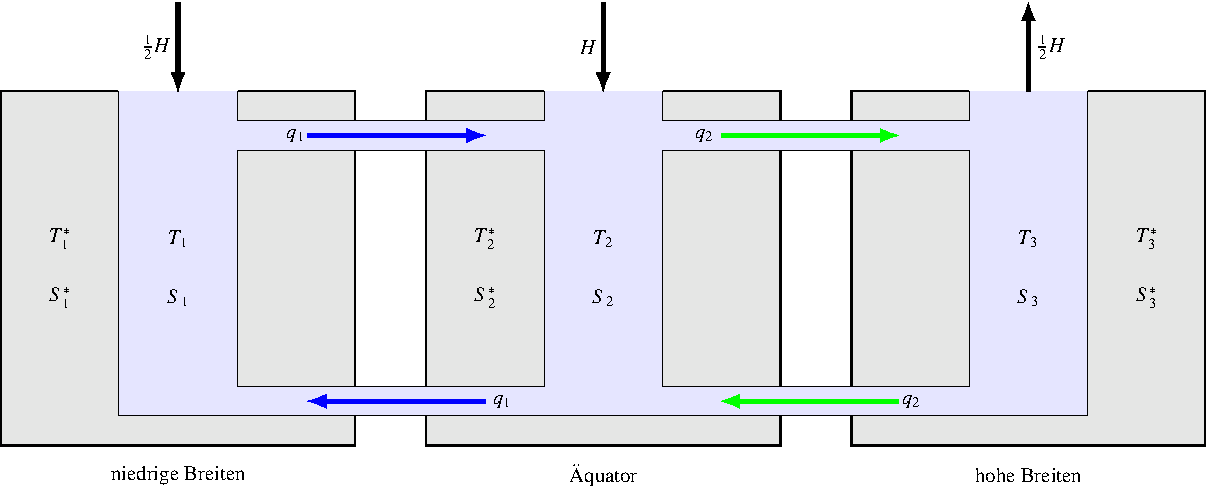
\includegraphics[width=14cm]{thermohalin/tikz/3b2f.pdf}
	\caption{Zwei-Fluss Modell des THC}
		\label{thermohalin:3b2f}
\end{figure}

So lassen sich nun für jede Box die zugehörigen Salinitäts- und Temperaturgleichungen aufstellen. So ist auch ersichtlich, dass Box $1$ und $3$ jeweils einen Fluss in der Gleichung haben. Im gegensatz dazu hat Box $2$ jedoch zwei Flüsse in der Gleichung. Das liegt daran, das wie aus der Abbildung ersichtlich, dass die mittlere Box von beiden Strömen durchflossen wird.


\begin{equation}
\begin{aligned}
\frac{dT_1}{dt} &= c(T_1^*-T_1)&+|q_1|(T_2-T_1)\phantom{+|q_2|(T_3-T_2)}
\\
\frac{dT_2}{dt} &= c(T_2^*-T_2)&+|q_1|(T_1-T_2)+|q_2|(T_3-T_2)
\\
\frac{dT_3}{dt} &= c(T_3^*-T_3)&+ \phantom{+|q_1|(T_1-T_2)}|q_2|(T_2-T_3)
\end{aligned}
\end{equation}
\begin{equation}
\begin{aligned}
\frac{dS_1}{dt} &= -H/2 &+ d(S_1^*-S_1)&+|q_1|(S_2-S_1)\phantom{+|q_2|(S_3-S_2)}
\\
\frac{dS_2}{dt} &= \phantom{-}H &+ d(S_2^*-S_2)&+|q_1|(S_1-S_2)+|q_2|(S_3-S_2)	
\\
\frac{dS_3}{dt} &= -H/2 &+d(S_3^*-S_3)&+ \phantom{+|q_1|(S_1-S_2)}|q_2|(S_2-S_3)
\end{aligned}
\end{equation}	

Dazu die Flussgleichungen die jeweils nur von den Dichtegradienten der jeweiligen Boxen abhängig sind:

\begin{equation}
\begin{aligned}
 q1 &= k[\alpha(T_2-T_1)-\beta(S_2-S_1)] 
 \\
 q2 &= k[\alpha(T_3-T_2)-\beta(S_3-S_2)]
\end{aligned}
\end{equation}

\subsubsection{Matlab-Code}

Erklärung des codes, Codeausschnitte

\subsubsection{Resultate}


Die Gleichungen sehen vielversprechend aus. Nur stimmen die Resulatate nicht mit der Realität überein.
Durch die entkoppelung der zwei Flüsse, war es möglich das der eine Seine Richtung ändert, der andere jedoch bleibt. Das resultiert in zwei gegenläufige Ströme welche in keiner Weise mit dem Golfstrom übereinstimmen.
Nachträglich ist dieser Fehler offensichtlich. Durch das Erlauben von zwei Flüssen Wird ermöglicht, dass in der Mitte euch eine auf- und Absteigzone entsteht.
diese Tatsache macht dieses Modell zu einem Fehlschlag.

%%input Matlab Graphen zur Darstellung der trennung und umkehrung der Zwei flüsse!!

\subsection{Ein-Fluss Modell} 

Dieses Modell ist der Nachfolger vom letzten. 
Um zu verhindern, dass in der mittleren Box eine zusätzliche Auf- und Absteigzone entsteht, muss dieser Weg verhindert werden. Das lässt sich erreichen, in dem die Äquatorzone nur für den Oberflächenfluss zugänglich ist. Der Tiefenfluss fliesst somit direkt von Pol zu Pol. 
Das lässt sich auch in der Realität nachweisen, Der Rückfluss tritt erst ausserhalb des Atlantik wieder an die Oberfläche.

\begin{figure}
	\centering
	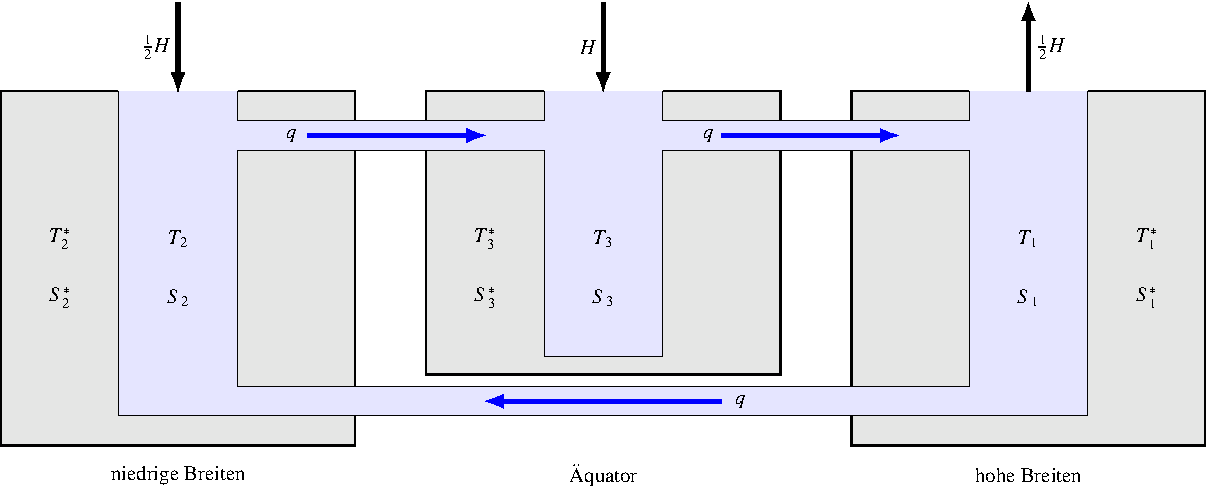
\includegraphics[width=14cm]{thermohalin/tikz/3b1f.pdf}
	\caption{Ein-Fluss Modell des THC}
	\label{thermohalin:3b1f}
\end{figure}

Aus diesem Modell lassen sich nun neue Gleichungen für die Boxen aufstellen:

\begin{equation}
\begin{aligned}
\frac{dT_1}{dt} &= c(T_p-T_1)&+ \begin{cases} q(T_3-T_1) & \quad q>0 \\ |q|(T_2-T_1) & \quad q<0 \end{cases}
\\
\frac{dT_2}{dt} &= c(T_p-T_2)&+\begin{cases} q(T_1-T_2) & \quad q>0 \\ |q|(T_3-T_2) & \quad q<0 \end{cases}
\\
\frac{dT_3}{dt} &= c(T_e-T_3)&+\begin{cases} q(T_2-T_3) & \quad q>0 \\ |q|(T_1-T_3) & \quad q<0 \end{cases}
\end{aligned}
\end{equation}
\begin{equation}
\begin{aligned}
\frac{dS_1}{dt} &= -H/2 &+ d(S_p-S_1)&+\begin{cases} q(S_3-S_1) & \quad q>0 \\ |q|(S_2-S_1) & \quad q<0 \end{cases}
\\
\frac{dS_2}{dt} &= \phantom{-}H &+ d(S_p-S_2)&+\begin{cases} q(S_1-S_2) & \quad q>0 \\ |q|(S_3-S_2) & \quad q<0 \end{cases}	
\\
\frac{dS_3}{dt} &= -H/2 &+d(S_e-S_3)&+\begin{cases} q(S_2-S_3) & \quad q>0 \\ |q|(S_1-S_3) & \quad q<0 \end{cases}
\end{aligned}
\end{equation}	
\subsubsection{Matlab-code}

Erklärung der Änderung, (Codeausschnitte)


\subsubsection{Resultate} 

1. Resultat normale Simulation mit aktuellen Werten

2. Simulation der werte nach klimaerwärmung

3. Vergleich Paper Liu Wei


